\documentclass{beamer}
\usepackage[utf8]{inputenc}

\usetheme{Madrid}
\usecolortheme{default}
\usepackage{amsmath,amssymb,amsfonts,amsthm}
\usepackage{txfonts}
\usepackage{tkz-euclide}
\usepackage{listings}
\usepackage{adjustbox}
\usepackage{array}
\usepackage{tabularx}
\usepackage{gvv}
\usepackage{lmodern}
\usepackage{circuitikz}
\usepackage{tikz}
\usepackage{graphicx}

\setbeamertemplate{page number in head/foot}[totalframenumber]

\usepackage{tcolorbox}
\tcbuselibrary{minted,breakable,xparse,skins}



\definecolor{bg}{gray}{0.95}
\DeclareTCBListing{mintedbox}{O{}m!O{}}{%
  breakable=true,
  listing engine=minted,
  listing only,
  minted language=#2,
  minted style=default,
  minted options={%
    linenos,
    gobble=0,
    breaklines=true,
    breakafter=,,
    fontsize=\small,
    numbersep=8pt,
    #1},
  boxsep=0pt,
  left skip=0pt,
  right skip=0pt,
  left=25pt,
  right=0pt,
  top=3pt,
  bottom=3pt,
  arc=5pt,
  leftrule=0pt,
  rightrule=0pt,
  bottomrule=2pt,

  colback=bg,
  colframe=orange!70,
  enhanced,
  overlay={%
    \begin{tcbclipinterior}
    \fill[orange!20!white] (frame.south west) rectangle ([xshift=20pt]frame.north west);
    \end{tcbclipinterior}},
  #3,
}
\lstset{
    language=C,
    basicstyle=\ttfamily\small,
    keywordstyle=\color{blue},
    stringstyle=\color{orange},
    commentstyle=\color{green!60!black},
    numbers=left,
    numberstyle=\tiny\color{gray},
    breaklines=true,
    showstringspaces=false,
}
%------------------------------------------------------------
%This block of code defines the information to appear in the
%Title page
\title %optional
{2.4.23}
\date{september 2025}
%\subtitle{A short story}

\author % (optional)
{J.NAVYASRI- EE25BTECH11028}

\begin{document}

\frame{\titlepage}
\begin{frame}{Question}
Do the points \( (3, 2) \), \( (-2, -3) \), and \( (2, 3) \) form a triangle? If so, name the type of triangle formed.
\end{frame}

% Step 1: Theoretical solution
\begin{frame}{Theoretical solution}
Given points,

\begin{equation}
A=\myvec{3\\2}, \quad 
B=\myvec{-2\\-3}, \quad 
C=\myvec{2\\3}
\end{equation}

\subsection*{1. Collinearity check (using rank)}

Form the matrix:
\begin{equation}
M=\myvec{
3 & 2 & 1\\
-2 & -3 & 1\\
2 & 3 & 1
}
\end{equation}

Apply row operations:
\begin{equation}
R_2 \leftarrow R_2+2R_1,\quad R_3 \leftarrow 3R_3-2R_1
\;\;\Rightarrow\;\;
\myvec{
3 & 2 & 1\\
4 & 1 & 3\\
0 & 5 & 1
}
\end{equation}

\begin{equation}
R_2 \leftarrow 3R_2-4R_1
\;\;\Rightarrow\;\;
\myvec{
3 & 2 & 1\\
0 & -5 & 5\\
0 & 5 & 1
}
\end{equation}
\end{frame}

% Step 2: Theoretical solution 
\begin{frame}{Theoretical solution}
\begin{equation}
R_3 \leftarrow R_3+R_2
\;\;\Rightarrow\;\;
\myvec{
3 & 2 & 1\\
0 & -5 & 5\\
0 & 0 & 6
}
\end{equation}

Since all three rows are nonzero:
\begin{equation}
\operatorname{rank}(M)=3
\end{equation}

\[
\Rightarrow \text{Points are not collinear, so they form a triangle.}
\]

\subsection*{2. Right-angle check}

\begin{equation}
\overrightarrow{AB}=B-A=\myvec{-5\\-5}, \quad 
\overrightarrow{AC}=C-A=\myvec{-1\\1}
\end{equation}
\end{frame}

% Step 3: Theoretical solution 
\begin{frame}{Theoretical solution}
\begin{equation}
\overrightarrow{AB}\cdot \overrightarrow{AC} = (-5)(-1)+(-5)(1)=0
\end{equation}

\[
\Rightarrow \overrightarrow{AB}\perp \overrightarrow{AC}
\]

So, the triangle is right-angled at
\begin{equation}
A=\myvec{3\\2}
\end{equation}

\subsection*{3. Final Answer}

\begin{equation}
\text{The given points form a triangle (rank = 3).}
\end{equation}

\begin{equation}
\text{The triangle is right-angled at } A=\myvec{3\\2}.
\end{equation}

\end{frame}

\begin{frame}[fragile]
    \frametitle{Python Code}
    \begin{lstlisting}
    import matplotlib.pyplot as plt

# Define the coordinates of the points
A = (3, 2)
B = (-2, -3)
C = (2, 3)

\end{lstlisting}
\end{frame}

\begin{frame}[fragile]
    \frametitle{Python Code}
    \begin{lstlisting}
    # Plot lines connecting the points
plt.plot([B[0], A[0]], [B[1], A[1]], 'b-')  # Line from B to A
plt.plot([B[0], C[0]], [B[1], C[1]], 'b-')  # Line from B to C
plt.plot([A[0], C[0]], [A[1], C[1]], 'b-')  # Line from A to C

# Plot the points themselves
plt.plot(A[0], A[1], 'ko')  # Point A
plt.plot(B[0], B[1], 'ko')  # Point B
plt.plot(C[0], C[1], 'ko')  # Point C

\end{lstlisting}
\end{frame}

\begin{frame}[fragile]
    \frametitle{Python Code}
    \begin{lstlisting}
# Add labels near the points
plt.text(A[0] + 0.1, A[1], 'A(3,2)')
plt.text(B[0] - 1.5, B[1], 'B(-2,-3)')
plt.text(C[0] - 1, C[1], 'C(2,3)')

# Axes labels
plt.xlabel('x')
plt.ylabel('y')

# Grid and central axes
plt.grid(True)
plt.axhline(0, color='black', linewidth=0.5)
plt.axvline(0, color='black', linewidth=0.5)

# Title and show plot
plt.title('Graph of Points A, B, C')
plt.show()


\end{lstlisting}
\end{frame}


\begin{frame}[fragile]
\frametitle{C Code}
\begin{lstlisting}
#include <stdio.h>
int main() {
    int x1=3,y1=2, x2=-2,y2=-3, x3=2,y3=3;

    int det = x1*(y2-y3) + x2*(y3-y1) + x3*(y1-y2);

    if(det==0)
        printf("The points are collinear. No triangle formed.\n");
    else
        printf("The points form a triangle.\n");

    return 0;
}


\end{lstlisting}

\end{frame}

\begin{frame}[fragile]
\frametitle{C Code}
\begin{lstlisting}
#include <stdio.h>
int main() {
    int x1=3,y1=2, x2=-2,y2=-3, x3=2,y3=3;

    int ABx=x2-x1, ABy=y2-y1;
    int ACx=x3-x1, ACy=y3-y1;
    int BCx=x3-x2, BCy=y3-y2;

    if(ABx*ACx + ABy*ACy == 0)
        printf("The triangle is right-angled at A(3,2).\n");
    else if(ABx*BCx + ABy*BCy == 0)
        printf("The triangle is right-angled at B(-2,-3).\n");
    else if(ACx*BCx + ACy*BCy == 0)
        printf("The triangle is right-angled at C(2,3).\n");

    return 0;
}


\end{lstlisting}

\end{frame}

\begin{frame}[fragile]
\frametitle{C Code}
\begin{lstlisting}
#include <stdio.h>
int main() {
    printf("Final Conclusion -> Triangle formed, right-angled at A(3,2).\n");
    return 0;
}

\end{lstlisting}

\end{frame}



    \begin{frame}[fragile]
\frametitle{Python and C Code}

\begin{lstlisting}
# PART 1: Input & Setup
x1, y1 = 3, 2
x2, y2 = -2, -3
x3, y3 = 2, 3
print("Points: A(3,2), B(-2,-3), C(2,3)")
\end{lstlisting}

\end{frame}

    \begin{frame}[fragile]
\frametitle{Python and C Code}

\begin{lstlisting}
# PART 2: Check Collinearity
x1,y1,x2,y2,x3,y3 = 3,2,-2,-3,2,3
det = x1*(y2-y3) + x2*(y3-y1) + x3*(y1-y2)
print("Collinear" if det==0 else "Not Collinear")

\end{lstlisting}

\end{frame}

    \begin{frame}[fragile]
\frametitle{Python and C Code}

\begin{lstlisting}
# PART 3: Check Right Angle
x1,y1,x2,y2,x3,y3 = 3,2,-2,-3,2,3
AB, AC, BC = (x2-x1,y2-y1), (x3-x1,y3-y1), (x3-x2,y3-y2)

if AB[0]*AC[0]+AB[1]*AC[1]==0: print("Right angle at A")
elif AB[0]*BC[0]+AB[1]*BC[1]==0: print("Right angle at B")
elif AC[0]*BC[0]+AC[1]*BC[1]==0: print("Right angle at C")
else: print("No right angle")
\end{lstlisting}

\end{frame}

    \begin{frame}[fragile]
\frametitle{Python and C Code}

\begin{lstlisting}
import matplotlib.pyplot as plt

# PART 4: Final Conclusion + Plot
x1,y1,x2,y2,x3,y3 = 3,2,-2,-3,2,3
X,Y = [x1,x2,x3,x1],[y1,y2,y3,y1]
plt.plot(X,Y,'bo-'); plt.grid(True); plt.gca().set_aspect('equal')
plt.text(x1+0.1,y1+0.1,"A"); plt.text(x2+0.1,y2+0.1,"B"); plt.text(x3+0.1,y3+0.1,"C")
plt.show()
\end{lstlisting}

\end{frame}



\textbf{Graphical Representation:}

\begin{center}
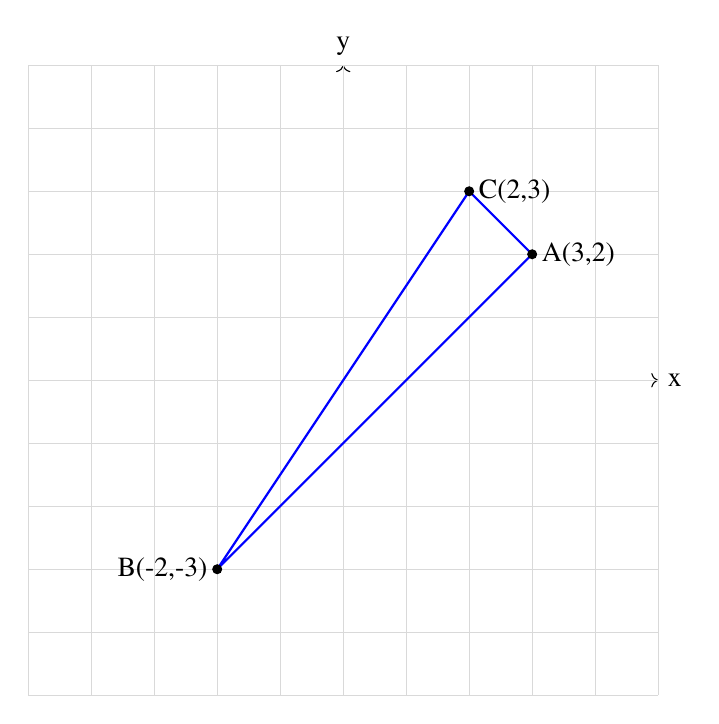
\begin{tikzpicture}[scale=0.8]
    % Draw axes
    \draw[->] (-5,0) -- (5,0) node[right] {x};
    \draw[->] (0,-5) -- (0,5) node[above] {y};

    % Grid (optional)
    \draw[step=1cm,gray!30,very thin] (-5,-5) grid (5,5);

    % Points
    \coordinate (A) at (3,2);
    \coordinate (B) at (-2,-3);
    \coordinate (C) at (2,3);

    % Draw triangle
    \draw[thick, blue] (A) -- (B) -- (C) -- cycle;

    % Draw and label points
    \filldraw[black] (A) circle (2pt) node[anchor=west] {A(3,2)};
    \filldraw[black] (B) circle (2pt) node[anchor=east] {B(-2,-3)};
    \filldraw[black] (C) circle (2pt) node[anchor=west] {C(2,3)};
    \end{tikzpicture}
    
        % Add "Fig. 0" text below the figure
    \vspace{0.5cm} % space between figure and text
    \textbf{Fig. 0}

\end{center}

\end{document}

